\documentclass{article}
\usepackage{graphicx}
\usepackage{caption}
\usepackage{subcaption}
\graphicspath{{./figs/}}{}
\usepackage{listings}
\title{
HLS-Assignment 2.3
}
\begin{document}
\maketitle
\hfill \textbf{Sampath Govardhan} \\
\null \hfill \textbf{FWC22071}\\
\tableofcontents
\section{Problem Statement}
\begin{lstlisting}
Repeat the experiment in Assignment 1 with the following change:
Repeat Assignment 2.1 and 2.2 with the change mentioned in Assignment 3.
Analyse change in timing report from Assignment 1, 2.1, 2.2, and report 
your understanding of why it changed. 
\end{lstlisting}
\vspace{10cm}


\section{Design Code}
\textbf{2.3.1}
\begin{lstlisting}
#include <iostream>
#include "hls_stream.h"


typedef int in;
typedef long out;

void mul(hls::stream<in> &x,hls::stream<in> &y,hls::stream<out> &z)
{

 in a,b;
 out c;
 a=x.read();
 b=y.read();
 c = a * b;
 z.write(c);
}

\end{lstlisting}
\vspace{2cm}
\textbf{2.3.2}
\begin{lstlisting}
#include <iostream>
#include "hls_stream.h"
#include "ap_fixed.h"

typedef ap_fixed<28,4> in;
typedef ap_fixed<56,8> out;

void mul(hls::stream<in> &x,hls::stream<in> &y,hls::stream<out> &z)
{

 in a,b;
 out c;
 a=x.read();
 b=y.read();
 c = a * b;
 z.write(c);
}


\end{lstlisting}
\vspace{5cm}


\section{Test Bench Code}
\textbf{2.3.1}
\begin{lstlisting}
#include <iostream>
#include "hls_stream.h"

using namespace std;

typedef int in;
typedef long out;

void mul(hls::stream<in> &x,hls::stream<in> &y,hls::stream<out> &z);
int main()
{
hls::stream<in> a,b;
hls::stream<out> c;

int i;

for (i=0;i<=9;i++){
a.write (i+1);
b.write (i+3);
mul(a,b,c);
cout << "\n" << c.read();
}
return 0;
}


\end{lstlisting}
\vspace{2cm}
\textbf{2.3.2}
\begin{lstlisting}
#include <iostream>
#include "hls_stream.h"
#include "ap_fixed.h"
using namespace std;

typedef ap_fixed<28,4> in;
typedef ap_fixed<56,8> out;

void mul(hls::stream<in> &x,hls::stream<in> &y,hls::stream<out> &z);
int main()
{
hls::stream<in> a,b;
hls::stream<out> c;

int i;

for (i=0;i<=9;i++){
a.write (i+0.456789875);
b.write (i);
mul(a,b,c);
cout << "\n" << c.read();
}
return 0;
}


\end{lstlisting}

\vspace{5cm}


\section{C Simulation Output}
\textbf{2.3.1}
\begin{lstlisting}
INFO: [SIM 2] *************** CSIM start ***************
INFO: [SIM 4] CSIM will launch GCC as the compiler.
   Compiling ../../../../cpp_ap_fixed.cpp in debug mode
   Generating csim.exe

3
8
15
24
35
48
63
80
99
120
INFO: [SIM 1] CSim done with 0 errors.
INFO: [SIM 3] *************** CSIM finish ***************


\end{lstlisting}
\vspace{2cm}
\textbf{2.3.2}
\begin{lstlisting}
INFO: [SIM 2] *************** CSIM start ***************
INFO: [SIM 4] CSIM will launch GCC as the compiler.
   Compiling ../../../../cpp_ap_fixed_test.cpp in debug mode
   Generating csim.exe

0
1.45679
4.91358
10.3704
17.8272
27.2839
38.7407
52.1975
60.3457
45.8025
INFO: [SIM 1] CSim done with 0 errors.
INFO: [SIM 3] *************** CSIM finish ***************


\end{lstlisting}
\vspace{10cm}

\section{HLS Resource Consumption}
\vspace{1cm}
\begin{figure}[h]
\centering
\begin{subfigure}[b]{0.8\textwidth}
    \centering
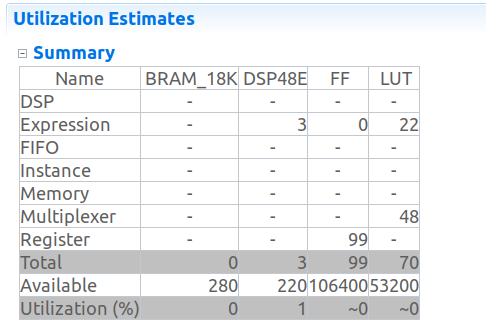
\includegraphics[width=\textwidth]{figs/31a.png}
    \caption{3.2.1}
    \label{fig:my_label}
\end{subfigure}
\hfill
\begin{subfigure}[b]{0.8\textwidth}
    \centering
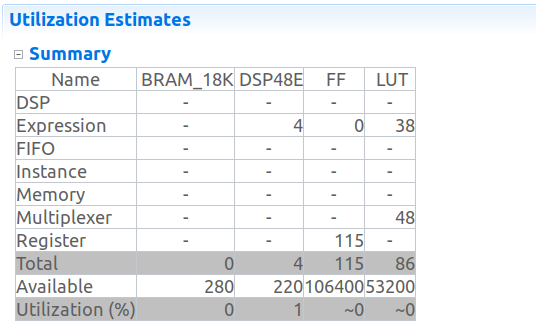
\includegraphics[width=\textwidth]{figs/31b.png}
    \caption{3.2.2}
    \label{fig:my_label}
\end{subfigure}
\end{figure}
\begin{lstlisting}
Here more resources are used compared to all previous Assignments this is
because by using Streaming Interfaces we use single master and single slave 
at a time to transmit or recieve data in a serial manner (Serial
Communication).
\end{lstlisting}
\vspace{5cm}


\section{HLS Timing Report}
\vspace{1cm}
\begin{figure}[h]
\centering
\begin{subfigure}[b]{0.8\textwidth}
    \centering
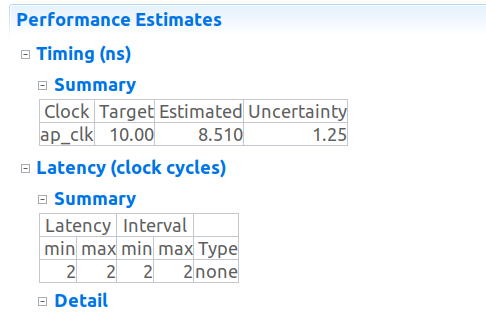
\includegraphics[width=\textwidth]{figs/32a.png}
    \caption{3.2.1}
    \label{fig:my_label}
\end{subfigure}
\hfill
\begin{subfigure}[b]{0.8\textwidth}
    \centering
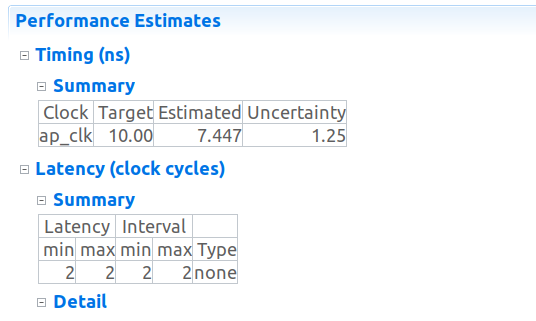
\includegraphics[width=\textwidth]{figs/32b.png}
    \caption{3.2.2}
    \label{fig:my_label}
\end{subfigure}
\end{figure}
\begin{lstlisting}
Here Timing remains same but Latency is changed compared to all previous
Assignments this is because by using Streaming Interfaces we changed our
Combinational logic into a Sequential logic thus takes 1 clock cycle to
produce overall output.
\end{lstlisting}
\vspace{5cm}


\section{Interfaces Report}
\vspace{1cm}
\begin{figure}[h]
\centering
\begin{subfigure}[b]{0.6\textwidth}
    \centering
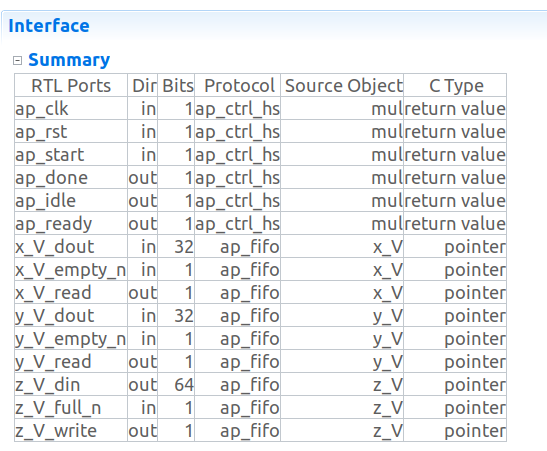
\includegraphics[width=\textwidth]{figs/33a.png}
    \caption{3.2.1}
    \label{fig:my_label}
\end{subfigure}
\hfill
\begin{subfigure}[b]{0.6\textwidth}
    \centering
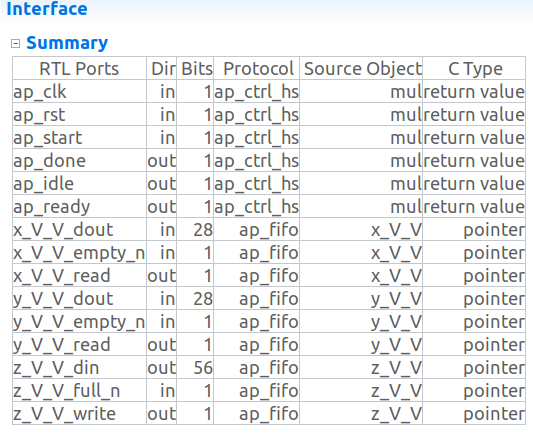
\includegraphics[width=\textwidth]{figs/33b.png}
    \caption{3.2.2}
    \label{fig:my_label}
\end{subfigure}
\end{figure}
\vspace{15cm}


\section{C/RTL Cosimulation Output}
\vspace{1cm}
\textbf{2.3.1}
\begin{lstlisting}

Starting C/RTL cosimulation ...
/tools/Xilinx/Vivado/2018.3/bin/vivado_hls /home/sam-admin/Xilinx/HLS/cpp_ap_fixed/proj_cpp_ap_fixed/solution1/cosim.tcl
INFO: [HLS 200-10] Running '/tools/Xilinx/Vivado/2018.3/bin/unwrapped/lnx64.o/vivado_hls'
INFO: [HLS 200-10] For user 'sam-admin' on host 'sampaths-lappie' (Linux_x86_64 version 5.19.0-35-generic) on Tue Mar 21 15:44:09 IST 2023
INFO: [HLS 200-10] On os Ubuntu 22.04.2 LTS
INFO: [HLS 200-10] In directory '/home/sam-admin/Xilinx/HLS/cpp_ap_fixed'
INFO: [HLS 200-10] Opening project '/home/sam-admin/Xilinx/HLS/cpp_ap_fixed/proj_cpp_ap_fixed'.
INFO: [HLS 200-10] Opening solution '/home/sam-admin/Xilinx/HLS/cpp_ap_fixed/proj_cpp_ap_fixed/solution1'.
INFO: [SYN 201-201] Setting up clock 'default' with a period of 10ns.
INFO: [HLS 200-10] Setting target device to 'xc7z020clg484-1'
INFO: [COSIM 212-47] Using XSIM for RTL simulation.
INFO: [COSIM 212-14] Instrumenting C test bench ...
   Build using "/tools/Xilinx/Vivado/2018.3/tps/lnx64/gcc-6.2.0/bin/g++"
   Compiling apatb_mul.cpp
   Compiling cpp_ap_fixed.cpp_pre.cpp.tb.cpp
   Compiling cpp_ap_fixed_test.cpp_pre.cpp.tb.cpp
   Generating cosim.tv.exe
INFO: [COSIM 212-302] Starting C TB testing ... 


3
8
15
24
35
48
63
80
99
120INFO: [COSIM 212-333] Generating C post check test bench ...
INFO: [COSIM 212-12] Generating RTL test bench ...
INFO: [COSIM 212-323] Starting verilog simulation. 
INFO: [COSIM 212-15] Starting XSIM ...
INFO: [XSIM 43-3496] Using init file passed via -initfile option "/tools/Xilinx/Vivado/2018.3/data/xsim/ip/xsim_ip.ini".
Vivado Simulator 2018.3
Copyright 1986-1999, 2001-2018 Xilinx, Inc. All Rights Reserved.
Running: /tools/Xilinx/Vivado/2018.3/bin/unwrapped/lnx64.o/xelab xil_defaultlib.apatb_mul_top glbl -prj mul.prj -L smartconnect_v1_0 -L axi_protocol_checker_v1_1_12 -L axi_protocol_checker_v1_1_13 -L axis_protocol_checker_v1_1_11 -L axis_protocol_checker_v1_1_12 -L xil_defaultlib -L unisims_ver -L xpm --initfile /tools/Xilinx/Vivado/2018.3/data/xsim/ip/xsim_ip.ini --lib ieee_proposed=./ieee_proposed -s mul 
Multi-threading is on. Using 6 slave threads.
WARNING: [XSIM 43-3431] One or more environment variables have been detected which affect the operation of the C compiler. These are typically not set in standard installations and are not tested by Xilinx, however they may be appropriate for your system, so the flow will attempt to continue.  If errors occur, try running xelab with the "-mt off -v 1" switches to see more information from the C compiler. The following environment variables have been detected:
    LIBRARY_PATH
INFO: [VRFC 10-2263] Analyzing SystemVerilog file "/home/sam-admin/Xilinx/HLS/cpp_ap_fixed/proj_cpp_ap_fixed/solution1/sim/verilog/glbl.v" into library work
INFO: [VRFC 10-311] analyzing module glbl
INFO: [VRFC 10-2263] Analyzing SystemVerilog file "/home/sam-admin/Xilinx/HLS/cpp_ap_fixed/proj_cpp_ap_fixed/solution1/sim/verilog/AESL_autofifo_y_V.v" into library xil_defaultlib
INFO: [VRFC 10-311] analyzing module AESL_autofifo_y_V
INFO: [VRFC 10-2263] Analyzing SystemVerilog file "/home/sam-admin/Xilinx/HLS/cpp_ap_fixed/proj_cpp_ap_fixed/solution1/sim/verilog/mul.v" into library xil_defaultlib
INFO: [VRFC 10-311] analyzing module mul
INFO: [VRFC 10-2263] Analyzing SystemVerilog file "/home/sam-admin/Xilinx/HLS/cpp_ap_fixed/proj_cpp_ap_fixed/solution1/sim/verilog/AESL_autofifo_x_V.v" into library xil_defaultlib
INFO: [VRFC 10-311] analyzing module AESL_autofifo_x_V
INFO: [VRFC 10-2263] Analyzing SystemVerilog file "/home/sam-admin/Xilinx/HLS/cpp_ap_fixed/proj_cpp_ap_fixed/solution1/sim/verilog/AESL_autofifo_z_V.v" into library xil_defaultlib
INFO: [VRFC 10-311] analyzing module AESL_autofifo_z_V
INFO: [VRFC 10-2263] Analyzing SystemVerilog file "/home/sam-admin/Xilinx/HLS/cpp_ap_fixed/proj_cpp_ap_fixed/solution1/sim/verilog/mul.autotb.v" into library xil_defaultlib
INFO: [VRFC 10-311] analyzing module apatb_mul_top
Starting static elaboration
Completed static elaboration
Starting simulation data flow analysis
Completed simulation data flow analysis
Time Resolution for simulation is 1ps
Compiling module xil_defaultlib.mul
Compiling module xil_defaultlib.AESL_autofifo_x_V
Compiling module xil_defaultlib.AESL_autofifo_y_V
Compiling module xil_defaultlib.AESL_autofifo_z_V
Compiling module xil_defaultlib.apatb_mul_top
Compiling module work.glbl
Built simulation snapshot mul


****** Webtalk v2018.3 (64-bit)
  **** SW Build 2405991 on Thu Dec  6 23:36:41 MST 2018
  **** IP Build 2404404 on Fri Dec  7 01:43:56 MST 2018
    ** Copyright 1986-2018 Xilinx, Inc. All Rights Reserved.


source /home/sam-admin/Xilinx/HLS/cpp_ap_fixed/proj_cpp_ap_fixed/solution1/sim/verilog/xsim.dir/mul/webtalk/xsim_webtalk.tcl -notrace
webtalk_transmit: Time (s): cpu = 00:00:00.58 ; elapsed = 00:00:06 . Memory (MB): peak = 388.926 ; gain = 0.000 ; free physical = 1311 ; free virtual = 6658
INFO: [Common 17-206] Exiting Webtalk at Tue Mar 21 15:44:25 2023...


****** xsim v2018.3 (64-bit)
  **** SW Build 2405991 on Thu Dec  6 23:36:41 MST 2018
  **** IP Build 2404404 on Fri Dec  7 01:43:56 MST 2018
    ** Copyright 1986-2018 Xilinx, Inc. All Rights Reserved.


source xsim.dir/mul/xsim_script.tcl
# xsim {mul} -autoloadwcfg -tclbatch {mul.tcl}
Vivado Simulator 2018.3
Time resolution is 1 ps
source mul.tcl
## run all
////////////////////////////////////////////////////////////////////////////////////
// Inter-Transaction Progress: Completed Transaction / Total Transaction
// Intra-Transaction Progress: Measured Latency / Latency Estimation * 100%
//
// RTL Simulation : "Inter-Transaction Progress" ["Intra-Transaction Progress"] @ "Simulation Time"
////////////////////////////////////////////////////////////////////////////////////
// RTL Simulation : 0 / 10 [0.00%] @ "125000"
// RTL Simulation : 1 / 10 [100.00%] @ "165000"
// RTL Simulation : 2 / 10 [100.00%] @ "195000"
// RTL Simulation : 3 / 10 [100.00%] @ "225000"
// RTL Simulation : 4 / 10 [100.00%] @ "255000"
// RTL Simulation : 5 / 10 [100.00%] @ "285000"
// RTL Simulation : 6 / 10 [100.00%] @ "315000"
// RTL Simulation : 7 / 10 [100.00%] @ "345000"
// RTL Simulation : 8 / 10 [100.00%] @ "375000"
// RTL Simulation : 9 / 10 [100.00%] @ "405000"
// RTL Simulation : 10 / 10 [100.00%] @ "435000"
////////////////////////////////////////////////////////////////////////////////////
$finish called at time : 475 ns : File "/home/sam-admin/Xilinx/HLS/cpp_ap_fixed/proj_cpp_ap_fixed/solution1/sim/verilog/mul.autotb.v" Line 329
## quit
INFO: [Common 17-206] Exiting xsim at Tue Mar 21 15:44:33 2023...
INFO: [COSIM 212-316] Starting C post checking ...


3
8
15
24
35
48
63
80
99
120INFO: [COSIM 212-1000] *** C/RTL co-simulation finished: PASS ***
Finished C/RTL cosimulation.



\end{lstlisting}
\vspace{2cm}
\textbf{2.3.2}
\begin{lstlisting}


Starting C/RTL cosimulation ...
/tools/Xilinx/Vivado/2018.3/bin/vivado_hls /home/sam-admin/Xilinx/HLS/cpp_ap_fixed/proj_cpp_ap_fixed/solution1/cosim.tcl
INFO: [HLS 200-10] Running '/tools/Xilinx/Vivado/2018.3/bin/unwrapped/lnx64.o/vivado_hls'
INFO: [HLS 200-10] For user 'sam-admin' on host 'sampaths-lappie' (Linux_x86_64 version 5.19.0-35-generic) on Tue Mar 21 15:52:09 IST 2023
INFO: [HLS 200-10] On os Ubuntu 22.04.2 LTS
INFO: [HLS 200-10] In directory '/home/sam-admin/Xilinx/HLS/cpp_ap_fixed'
INFO: [HLS 200-10] Opening project '/home/sam-admin/Xilinx/HLS/cpp_ap_fixed/proj_cpp_ap_fixed'.
INFO: [HLS 200-10] Opening solution '/home/sam-admin/Xilinx/HLS/cpp_ap_fixed/proj_cpp_ap_fixed/solution1'.
INFO: [SYN 201-201] Setting up clock 'default' with a period of 10ns.
INFO: [HLS 200-10] Setting target device to 'xc7z020clg484-1'
INFO: [COSIM 212-47] Using XSIM for RTL simulation.
INFO: [COSIM 212-14] Instrumenting C test bench ...
   Build using "/tools/Xilinx/Vivado/2018.3/tps/lnx64/gcc-6.2.0/bin/g++"
   Compiling apatb_mul.cpp
   Compiling cpp_ap_fixed.cpp_pre.cpp.tb.cpp
   Compiling cpp_ap_fixed_test.cpp_pre.cpp.tb.cpp
   Generating cosim.tv.exe
INFO: [COSIM 212-302] Starting C TB testing ... 


0
1.45679
4.91358
10.3704
17.8272
27.2839
38.7407
52.1975
60.3457
45.8025INFO: [COSIM 212-333] Generating C post check test bench ...
INFO: [COSIM 212-12] Generating RTL test bench ...
INFO: [COSIM 212-323] Starting verilog simulation. 
INFO: [COSIM 212-15] Starting XSIM ...
INFO: [XSIM 43-3496] Using init file passed via -initfile option "/tools/Xilinx/Vivado/2018.3/data/xsim/ip/xsim_ip.ini".
Vivado Simulator 2018.3
Copyright 1986-1999, 2001-2018 Xilinx, Inc. All Rights Reserved.
Running: /tools/Xilinx/Vivado/2018.3/bin/unwrapped/lnx64.o/xelab xil_defaultlib.apatb_mul_top glbl -prj mul.prj -L smartconnect_v1_0 -L axi_protocol_checker_v1_1_12 -L axi_protocol_checker_v1_1_13 -L axis_protocol_checker_v1_1_11 -L axis_protocol_checker_v1_1_12 -L xil_defaultlib -L unisims_ver -L xpm --initfile /tools/Xilinx/Vivado/2018.3/data/xsim/ip/xsim_ip.ini --lib ieee_proposed=./ieee_proposed -s mul 
Multi-threading is on. Using 6 slave threads.
WARNING: [XSIM 43-3431] One or more environment variables have been detected which affect the operation of the C compiler. These are typically not set in standard installations and are not tested by Xilinx, however they may be appropriate for your system, so the flow will attempt to continue.  If errors occur, try running xelab with the "-mt off -v 1" switches to see more information from the C compiler. The following environment variables have been detected:
    LIBRARY_PATH
INFO: [VRFC 10-2263] Analyzing SystemVerilog file "/home/sam-admin/Xilinx/HLS/cpp_ap_fixed/proj_cpp_ap_fixed/solution1/sim/verilog/glbl.v" into library work
INFO: [VRFC 10-311] analyzing module glbl
INFO: [VRFC 10-2263] Analyzing SystemVerilog file "/home/sam-admin/Xilinx/HLS/cpp_ap_fixed/proj_cpp_ap_fixed/solution1/sim/verilog/AESL_autofifo_y_V_V.v" into library xil_defaultlib
INFO: [VRFC 10-311] analyzing module AESL_autofifo_y_V_V
INFO: [VRFC 10-2263] Analyzing SystemVerilog file "/home/sam-admin/Xilinx/HLS/cpp_ap_fixed/proj_cpp_ap_fixed/solution1/sim/verilog/mul.v" into library xil_defaultlib
INFO: [VRFC 10-311] analyzing module mul
INFO: [VRFC 10-2263] Analyzing SystemVerilog file "/home/sam-admin/Xilinx/HLS/cpp_ap_fixed/proj_cpp_ap_fixed/solution1/sim/verilog/AESL_autofifo_x_V_V.v" into library xil_defaultlib
INFO: [VRFC 10-311] analyzing module AESL_autofifo_x_V_V
INFO: [VRFC 10-2263] Analyzing SystemVerilog file "/home/sam-admin/Xilinx/HLS/cpp_ap_fixed/proj_cpp_ap_fixed/solution1/sim/verilog/mul.autotb.v" into library xil_defaultlib
INFO: [VRFC 10-311] analyzing module apatb_mul_top
INFO: [VRFC 10-2263] Analyzing SystemVerilog file "/home/sam-admin/Xilinx/HLS/cpp_ap_fixed/proj_cpp_ap_fixed/solution1/sim/verilog/AESL_autofifo_z_V_V.v" into library xil_defaultlib
INFO: [VRFC 10-311] analyzing module AESL_autofifo_z_V_V
Starting static elaboration
Completed static elaboration
Starting simulation data flow analysis
Completed simulation data flow analysis
Time Resolution for simulation is 1ps
Compiling module xil_defaultlib.mul
Compiling module xil_defaultlib.AESL_autofifo_x_V_V
Compiling module xil_defaultlib.AESL_autofifo_y_V_V
Compiling module xil_defaultlib.AESL_autofifo_z_V_V
Compiling module xil_defaultlib.apatb_mul_top
Compiling module work.glbl
Built simulation snapshot mul


****** Webtalk v2018.3 (64-bit)
  **** SW Build 2405991 on Thu Dec  6 23:36:41 MST 2018
  **** IP Build 2404404 on Fri Dec  7 01:43:56 MST 2018
    ** Copyright 1986-2018 Xilinx, Inc. All Rights Reserved.


source /home/sam-admin/Xilinx/HLS/cpp_ap_fixed/proj_cpp_ap_fixed/solution1/sim/verilog/xsim.dir/mul/webtalk/xsim_webtalk.tcl -notrace
INFO: [Common 17-206] Exiting Webtalk at Tue Mar 21 15:52:52 2023...


****** xsim v2018.3 (64-bit)
  **** SW Build 2405991 on Thu Dec  6 23:36:41 MST 2018
  **** IP Build 2404404 on Fri Dec  7 01:43:56 MST 2018
    ** Copyright 1986-2018 Xilinx, Inc. All Rights Reserved.


source xsim.dir/mul/xsim_script.tcl
# xsim {mul} -autoloadwcfg -tclbatch {mul.tcl}
Vivado Simulator 2018.3
Time resolution is 1 ps
source mul.tcl
## run all
////////////////////////////////////////////////////////////////////////////////////
// Inter-Transaction Progress: Completed Transaction / Total Transaction
// Intra-Transaction Progress: Measured Latency / Latency Estimation * 100%
//
// RTL Simulation : "Inter-Transaction Progress" ["Intra-Transaction Progress"] @ "Simulation Time"
////////////////////////////////////////////////////////////////////////////////////
// RTL Simulation : 0 / 10 [0.00%] @ "125000"
// RTL Simulation : 1 / 10 [100.00%] @ "165000"
// RTL Simulation : 2 / 10 [100.00%] @ "195000"
// RTL Simulation : 3 / 10 [100.00%] @ "225000"
// RTL Simulation : 4 / 10 [100.00%] @ "255000"
// RTL Simulation : 5 / 10 [100.00%] @ "285000"
// RTL Simulation : 6 / 10 [100.00%] @ "315000"
// RTL Simulation : 7 / 10 [100.00%] @ "345000"
// RTL Simulation : 8 / 10 [100.00%] @ "375000"
// RTL Simulation : 9 / 10 [100.00%] @ "405000"
// RTL Simulation : 10 / 10 [100.00%] @ "435000"
////////////////////////////////////////////////////////////////////////////////////
$finish called at time : 475 ns : File "/home/sam-admin/Xilinx/HLS/cpp_ap_fixed/proj_cpp_ap_fixed/solution1/sim/verilog/mul.autotb.v" Line 329
## quit
INFO: [Common 17-206] Exiting xsim at Tue Mar 21 15:53:00 2023...
INFO: [COSIM 212-316] Starting C post checking ...


0
1.45679
4.91358
10.3704
17.8272
27.2839
38.7407
52.1975
60.3457
45.8025INFO: [COSIM 212-1000] *** C/RTL co-simulation finished: PASS ***
Finished C/RTL cosimulation.

\end{lstlisting}
\vspace{15cm}


\section{C/RTL Cosimulation Report}
\vspace{1cm}
\begin{figure}[h]
\centering
\begin{subfigure}[b]{0.8\textwidth}
    \centering
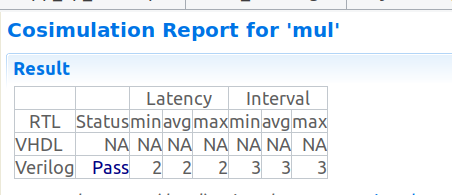
\includegraphics[width=\textwidth]{figs/34a.png}
    \caption{3.2.1}
    \label{fig:my_label}
\end{subfigure}
\hfill
\begin{subfigure}[b]{0.8\textwidth}
    \centering
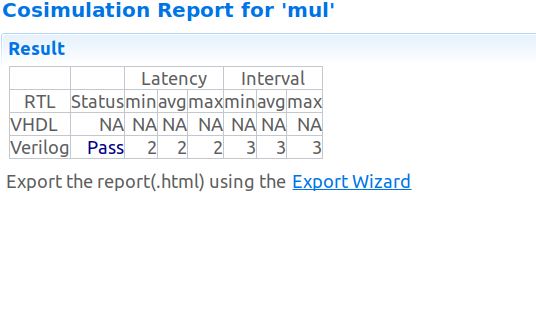
\includegraphics[width=\textwidth]{figs/34b.png}
    \caption{3.2.2}
    \label{fig:my_label}
\end{subfigure}
\end{figure}
\end{document}
